\documentclass[../main.tex]{subfiles}

\begin{document}

\subsection{High-Level Overview}

Figure \ref{fig:project_structure} demonstrates the structure of EngSci Press project. As explained in Section \ref{ssec:languages}, I coded the core dictionary in C and the story writer in Python. Users can customize both parts with \texttt{.txt} scripts.

\begin{figure}
	\centering
	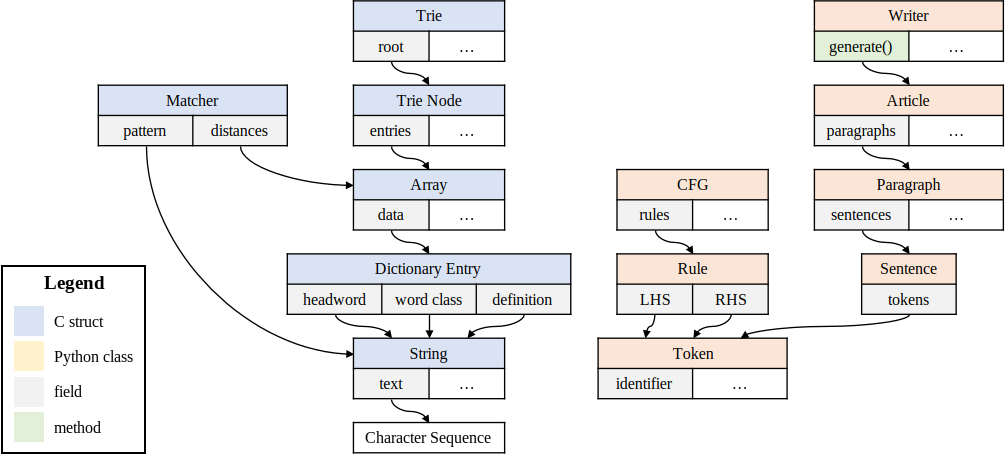
\includegraphics[scale=0.6]{project_structure}
	\caption{Overview of the project structure. Some fields and methods are omitted.}
	\label{fig:project_structure}
\end{figure}

\subsection{Languages}
\label{ssec:languages}

I use C for the core dictionary because it runs faster and provides more precise memory control. I initially wrote it in Python, but it took 3 seconds to launch and violated the time constraint. The bottleneck turns out to be CPU computation as opposed to disk IO. Moving to C should effectively speed it up since compiled languages typically compute much faster than interpreted languages \cite{bib:compiled_vs_interpreted}.

I use Python for the story writer because it is bot only easier to code, but also supports regular expression and features various sampling methods \cite{bib:numpy_sampling}. Usage of these functionalities is described in Section \ref{ssec:algorithms}. Python libraries such as NumPy have a mature and efficient C/Fortran back-end \cite{bib:numpy_source_code}. Compared to reinvented wheels, they are faster, more robust and easier to debug. Moreover, exception mechanism in Python makes it simpler to handle special cases that appear in a natural language.

\subsection{Data Structures}

\subsubsection{Dynamic Array}

Many functions in EngSci Press require a resizable and contiguous array. The most straightforward implementation is a block memory which is reallocated on each resize. However, frequent \texttt{realloc}s slow down the program \cite{bib:realloc_cost}. To achieve a balance between fewer \texttt{realloc}s and more compact storage, my custom \texttt{Array} type applies an exponential resizing strategy. It reserves more memory than its actual size. As shown in Figure \ref{fig:dynamic_array}, the memory space doubles when $\textrm{size} \geq \textrm{capacity}$ and halves when $\textrm{size} \leq \textrm{capacity} / 2$. A similar strategy is used for the \texttt{String} type.

\begin{figure}
	\centering
	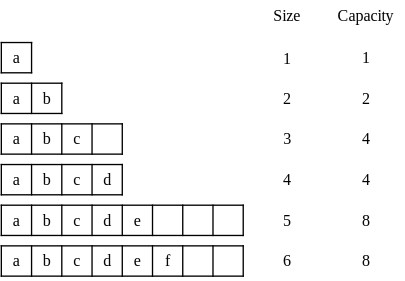
\includegraphics{dynamic_array}
	\caption{A dynamic array reserves space for future expansion.}
	\label{fig:dynamic_array}
\end{figure}

For convenience, an \texttt{Array} of pointers is designed to hold an optional destructor and execute it upon every element deletion. The destructor function frees all the memory that an element uses, both directly and indirectly.

\subsubsection{Trie}

I choose trie to store, access and modify dictionary data due to its efficiency \cite{bib:trie_efficiency} and convenience for implementation. Trie is a tree-like data structure that implements mapping with string keys. As shown in Figure \ref{fig:trie}, each node holds a single character. The key of a node is represented by the character sequence along the root-node path.

\begin{figure}
	\centering
	\includegraphics{trie}
	\caption{A trie. Each shadowed node represents an English word.}
	\label{fig:trie}
\end{figure}

Headwords are lower-cased as keys of dictionary entries, enabling case-insensitive search. Moreover, keys accept only characters whose ASCII codes fall in 32--64 or 97--122, because others are either upper-cased, or meaningless to appear in a dictionary headword. As a result, a trie node has 59 children at most.

For simplicity, mapping from a node to its children is implemented with a 59-element array of ordered child pointers. Fill \texttt{NULL} if a child does not exist. Such primitive implementation seems to affect performance negatively at first glance, as one has to check for many null pointers. However, because the accepted character set is small, a more advanced data structure, such as BST, usually brings more overhead as opposed to efficiency.

\subsubsection{Levenshtein Automaton}

EngSci Press uses edit distance \cite{bib:edit_distance} to measure the similarity between two strings. A Levenshtein automaton, constructed from a pattern string, can find the key which is most similar to the pattern from a trie. Such automaton is efficient \cite{bib:levenshtein_automaton} because it skips most of the trie branches which can be identified as non-matching.

Levenshtein automaton calculates edit distance by filling out a comparison matrix, as shown in Figure \ref{fig:edit_distance}. The matrix is $1 \times n$ when it starts searching ($n$ is the pattern string length). It pushes a character and fills a new row before it searches down a trie branch and pops them on leaving. The minimum of the $i$th row must be greater than or equal to the $(i-1)$th row. Therefore, the automaton quits when minimum of the last row exceeds its edit distance tolerance, since any further search only increases the distance even more.

\begin{figure}
		\centering
		\begin{tabular}{|c|c|c|c|c|c|c|c|}
			\hline
			& $\varnothing$ & \textbf{e} & \textbf{n} & \textbf{g} & \textbf{s} & \textbf{c} & \textbf{i} \\
			\hline
			$\varnothing$ & 0 & 1 & 2 & 3 & 4 & 5 & 6 \\
			\hline
			\textbf{e} & 1 & 0 & 1 & 2 & 3 & 4 & 5 \\
			\hline
			\textbf{n} & 2 & 1 & 0 & 1 & 2 & 3 & 4 \\
			\hline
			\textbf{s} & 3 & 2 & 1 & 1 & 1 & 2 & 3 \\
			\hline
			\textbf{i} & 4 & 3 & 2 & 2 & 2 & 2 & 2 \\
			\hline
			\textbf{g} & 5 & 4 & 3 & 2 & 3 & 3 & 3 \\
			\hline
			\textbf{n} & 6 & 5 & 4 & 3 & 3 & 4 & 4 \\
			\hline
		\end{tabular}
		\caption{Matrix that calculates the edit distance between ``engsci'' and ``ensign''.}
		\label{fig:edit_distance}
\end{figure}

\subsection{Algorithms}
\label{ssec:algorithms}

\subsubsection{Context-Free Grammar}

EngSci Press Grammar (ESPG) is a context-free grammar (CFG) \cite{bib:context_free_grammar} that generates English sentences. A CFG contains a start symbol (S) and describes many rewriting rules. The left-hand side (LHS) of a rule is a single token, and the right-hand side (RHS) is a sequence of one or more tokens. The rewriting process terminates when all tokens become English words (or terminals).

Stricter grammars such as regular grammar are not descriptive enough for a natural language \cite{bib:regular_grammar}, while more flexible ones can be challenging to implement for a generative purpose. For example, context-sensitive grammars, with more than one token on the LHS, can easily go into a blind alley, making it impossible to substitute all non-terminals.

Describing CFG with a Python \texttt{dict} is not hard, but wordy. To make my grammar more readable and maintainable, I design a simple description syntax as shown in Figure \ref{fig:cfg_description_syntax}. The text is parsed with \texttt{re} (regular expression) module and expanded into a \texttt{class CFG} instance. To make the output more natural, this syntax supports optional tokens (i.e.\ RHS tokens that can be omitted by a specified percentage chance) and weighted rules (i.e.\ with the same LHS, one rule has a higher execution chance than another).

\begin{figure}
	\centering
	\begin{lstlisting}[gobble=4]
		convergence = 0.3
		S -> NP VP "."
		0.9: NP -> Det (0.6: Adj) N
		0.1: NP -> NP "and" NP
		0.3: VP -> V NP
		0.6: VP -> V
		Det -> "the"
		Adj -> "smart"
		N -> "student"
		V -> "walks"
	\end{lstlisting}
	\vspace{-0.15in}
	\caption{Simple demonstration of the CFG description syntax.}
	\label{fig:cfg_description_syntax}
\end{figure}

\subsubsection{Story Length Control}

Properties of a CFG determine the length distribution of its generated sentences. CFG rules can be recursive \cite{bib:recursive_grammar}, where the LHS token appears on the RHS. Such rules, as $A \mapsto A B$, have a risk of falling into infinite loops: $A \mapsto A B \mapsto A B B \mapsto A B B B \mapsto \cdots$. A primitive yet effective patch for this is to set a convergence factor $\alpha$ \cite{bib:convergence_factor}. Weight of a rule decreases by $\alpha$ on each execution. As a result, non-recursive rules are preferred as a sentence grows longer, resulting in a finite output.

When generating an article, users might also want to specify the word/paragraph count. However, imagine every paragraph has exactly the same number of sentences -- such uniformity prevents the output from being non-human-like. To address this issue, EngSci Press determines the paragraph length by Poisson sampling, given the fact that lengths of human writings roughly follow a Poisson distribution. Parameter $\lambda$ of this distribution is user-defined, which is an indirect way to control story length.

\end{document}